\documentclass{beamer}
\usepackage[utf8]{inputenc}
\usepackage[brazil]{babel}
\usepackage{graphicx}
\usepackage{amsmath}
\usepackage{amsfonts}
\usepackage{amssymb}
\usepackage{tikz}
\usepackage{booktabs}
\usepackage{siunitx}
\usepackage{tabularx}
\usetikzlibrary{shapes, arrows, positioning}

% --- Configurações Globais ---
\usetheme{Warsaw}
\usecolortheme{default}
\setbeamertemplate{caption}[numbered]
\setbeameroption{show notes} 

% --- Informações do Documento ---
\title[Controle de Reator Químico]{Análise e Projeto de Sistemas de Controle para Reator Químico}
\subtitle{Estudo Comparativo de Técnicas de Controle}
\author{Lucas William Junges}
\institute{Universidade Federal de Santa Catarina (UFSC)}
\date{\today}

\begin{document}

% --- Slide de Título ---
\begin{frame}
    \titlepage
    \note{Apresentação do trabalho sobre o controle de um reator químico, explorando diferentes estratégias de controle, desde as mais simples até as mais avançadas.}
\end{frame}

% --- Roteiro ---
\begin{frame}{Roteiro da Apresentação}
    \tableofcontents
    \note{Este é o roteiro da nossa discussão. Começaremos com o problema, passaremos pela modelagem, exploraremos três abordagens de controle e finalizaremos com as conclusões.}
\end{frame}

\section{O Problema e a Modelagem}

% --- O Problema ---
\begin{frame}{O Problema: Controlando uma "Fábrica" Química}
    \large \textbf{Nosso Objetivo Principal:}
    \vspace{0.5em}
    
    \begin{columns}[T]
        \begin{column}{0.6\textwidth}
            \normalsize
            Controlar um reator químico (CSTR) que produz cyclopentenol. A meta é manter a \textbf{concentração do produto final (\(C_b\))} em um nível ideal, automaticamente.
            
            \vspace{0.5em}
            \alert{A Missão:} Projetar um controlador que ajuste a \textbf{vazão de diluição (\(u\))} para corrigir desvios e anular o efeito de \textbf{perturbações na entrada (\(C_{af}\))}.
        \end{column}
        \begin{column}{0.4\textwidth}
            \begin{figure}
                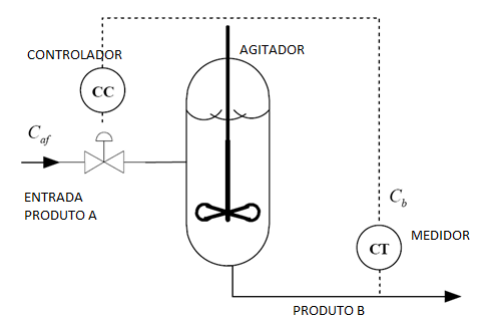
\includegraphics[width=0.9\textwidth]{Imagens/Reator.png}
                \caption{\tiny O Reator Químico (CSTR).}
            \end{figure}
        \end{column}
    \end{columns}
    \note{Aqui, definimos o problema central: manter a qualidade do produto estável, mesmo quando as condições de entrada variam. Apresentamos os três elementos-chave: a meta (saída), o ajuste (entrada) e o vilão (perturbação).}
\end{frame}

% --- Modelagem ---
\begin{frame}{A "Receita": Entendendo a Dinâmica do Processo}
    \small
    A dinâmica do processo é descrita por reações químicas e equações diferenciais.
    
    \textbf{Reações Químicas:}
    \begin{align*}
        A \xrightarrow{k_1} B & \quad \text{\tiny (Produto)} \\
        2A \xrightarrow{k_3} D & \quad \text{\tiny (Subproduto)}
    \end{align*}
    
    \textbf{Equações de Estado:}
    \tiny
    \begin{align*}
    \frac{dC_a}{dt} &= -k_1 C_a - k_3 C_a^2 + u(C_{af} - C_a) \\
    \frac{dC_b}{dt} &= k_1 C_a - k_2 C_b - u C_b
    \end{align*}
    \normalsize
    Este é um sistema \textbf{não linear}, cujo comportamento muda com as condições de operação.
    
    \note{Apresentamos o modelo matemático. É crucial entender que o sistema é não linear, e é por isso que a linearização se torna uma ferramenta importante para o projeto de controladores clássicos.}
\end{frame}

\section{Estratégias de Controle}

% --- Parte I: PI ---
\begin{frame}{Parte I: A Solução Clássica (Controlador PI)}
    \large \textbf{Abordagem:} Linearizar o sistema e projetar um controlador PI.
    \vspace{0.5em}
    
    \small
    \textbf{1. Linearização:} O modelo é simplificado em torno de um ponto de operação (\(C_{af}=5.1\), \(u=1\)) para se obter uma aproximação linear.
    
    \textbf{2. Projeto do PI:} Com a técnica de \textbf{alocação de polos}, projetamos um controlador para atender aos critérios de desempenho (\(t_{5\%} \in [1.5, 1.7]\) min, pico \(< 5\%\)).
    
    \textbf{Controlador:} \tiny \( C(s) = 1.85162 \frac{s + 1.91627}{s} \)
    
    \begin{figure}
        \centering
        \includegraphics[width=0.45\textwidth]{"Trabalho 1 Sistemas de Controle/respostacompequenasvariaçoes".png}
        \caption{\tiny Resposta do sistema com controlador PI.}
    \end{figure}
    
    \note{Explicamos a primeira abordagem: a mais simples e direta. Linearizamos o modelo para poder aplicar técnicas clássicas e projetamos um controlador PI. O resultado é bom, mas apenas perto do ponto onde linearizamos.}
\end{frame}

% --- Parte II: LR + FF ---
\begin{frame}{Parte II: A Solução Inteligente (LR + Feedforward)}
    \large \textbf{Abordagem:} Melhorar o desempenho com um controlador mais robusto e uma estratégia preditiva.
    \vspace{0.5em}
    
    \small
    \textbf{1. Controlador por Lugar das Raízes (LR):} Projetamos um controlador mais sofisticado para a função de transferência de 2ª ordem, resultando em uma resposta mais suave.
    \tiny \[ C(s)=\frac{5.2946(s+3.835)^2}{s(s+20)} \]
    
    \vspace{0.5em}
    \small
    \textbf{2. Controle Feedforward:} Para combater a perturbação (\(C_{af}\)) proativamente, nós a medimos e usamos essa informação para ajustar a entrada e anular seu efeito.
    
    \begin{figure}
        \includegraphics[width=0.3\textwidth]{"Trabalho 2 Sistemas de Controle/image3".png}
        \includegraphics[width=0.3\textwidth]{"Trabalho 2 Sistemas de Controle/image2".png}
        \caption{\tiny Desempenho sem (esquerda) e com (direita) Feedforward.}
    \end{figure}
    
    \note{Aqui, damos um passo à frente. O controlador por LR é mais adaptado à dinâmica do sistema. O grande salto de qualidade vem com o Feedforward, que nos permite anular a perturbação de forma muito eficaz.}
\end{frame}

% --- Parte III: Preditor de Smith ---
\begin{frame}{Parte III: Lidando com o Mundo Real (Atraso de Medição)}
    \large \textbf{Abordagem:} Compensar um atraso de 3 minutos na medição.
    \vspace{0.5em}
    
    \small
    \textbf{O Problema:} Atrasos na medição são comuns e podem desestabilizar o sistema, pois o controlador reage a uma informação "velha".
    
    \vspace{0.5em}
    
    \textbf{A Solução: Preditor de Smith.} Esta técnica usa um modelo do processo para "prever" a saída \textit{sem} o atraso. O controlador reage à previsão, não à medição atrasada, contornando o problema.
    
    \begin{figure}
        \centering
        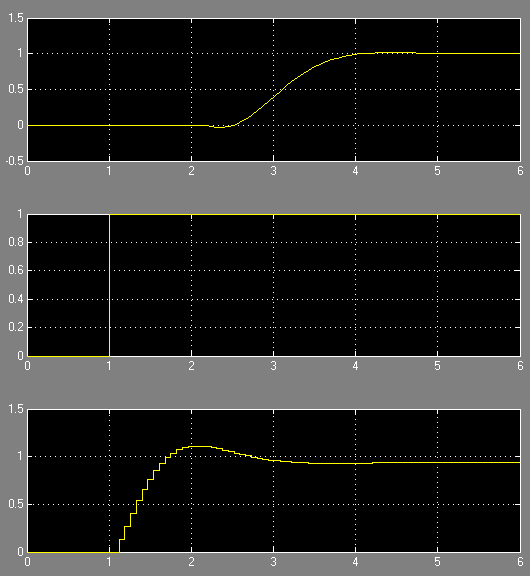
\includegraphics[width=0.25\textwidth]{Imagens/q13.png}
        \caption{\tiny Estrutura do Preditor de Smith.}
    \end{figure}
    
    \note{Este é o desafio mais realista. Atrasos são um grande problema em controle de processos. O Preditor de Smith é uma solução elegante que nos permite usar o controlador que já projetamos, adicionando uma camada de "previsão" para compensar o atraso.}
\end{frame}

% --- Comparativo Visual ---
\begin{frame}{Quadro Comparativo das Estratégias de Controle}
    \centering
    \tiny
    \renewcommand{\arraystretch}{1.1}
    \begin{tabularx}{\textwidth}{|X|X|X|X|}
        \hline
        \textbf{Estratégia} & \textbf{Princípio} & \textbf{Prós} & \textbf{Contras} \\
        \hline
        PI Clássico & Linearização e controle PI & Simples, robusto, fácil implementação & Eficaz só perto do ponto de operação, desempenho limitado \\
        \hline
        LR + Feedforward & Alocação de polos + ação preditiva & Excelente rejeição a perturbações, desempenho superior & Mais complexo, requer sensor extra, maior custo \\
        \hline
        Preditor de Smith & Compensação de atraso via modelo & Essencial para sistemas com atraso, mantém desempenho & Depende da precisão do modelo, sensível a erros de atraso \\
        \hline
    \end{tabularx}
    \note{Este quadro facilita a comparação direta das estratégias, ajudando a escolher a mais adequada para cada situação. Use este slide para reforçar os pontos-chave antes das conclusões.}
\end{frame}

% --- Aplicação Ideal ---
\begin{frame}{Aplicação Ideal de Cada Estratégia}
    \begin{itemize}
        \item \textbf{PI:} Processos estáveis, sem grandes perturbações ou atrasos.
        \item \textbf{LR+FF:} Processos sujeitos a perturbações mensuráveis.
        \item \textbf{Smith:} Processos com atraso de medição relevante.
    \end{itemize}
    \note{Este slide separa a aplicação ideal de cada estratégia, tornando a apresentação mais limpa e evitando excesso de conteúdo em um único frame.}
\end{frame}

\section{Conclusões}

% --- Conclusões ---
\begin{frame}[allowframebreaks]{Conclusões: Qual a Melhor Estratégia?}
    \large Não existe uma única resposta. A escolha ideal depende do balanço entre \textbf{desempenho, complexidade e custo}.
    
    \vspace{1em}
    
    \begin{itemize}
        \item \textbf{Controlador PI (Parte I):}
        \begin{itemize}
            \item \small \textbf{Prós:} Simples de projetar e implementar. Robusto.
            \item \small \textbf{Contras:} Desempenho limitado, eficaz apenas perto do ponto de operação.
        \end{itemize}
        
        \vspace{0.5em}
        
        \item \textbf{LR + Feedforward (Parte II):}
        \begin{itemize}
            \item \small \textbf{Prós:} Desempenho muito superior, excelente rejeição a perturbações.
            \item \small \textbf{Contras:} Mais complexo de projetar. Requer um sensor adicional para medir a perturbação (mais caro).
        \end{itemize}
        
        \vspace{0.5em}
        
        \item \textbf{Preditor de Smith (Parte III):}
        \begin{itemize}
            \item \small \textbf{Prós:} Essencial para sistemas com atraso, recuperando o desempenho.
            \item \small \textbf{Contras:} O desempenho depende da precisão do modelo. Erros na estimativa do atraso podem degradar a resposta.
        \end{itemize}
    \end{itemize}
    
    \note{Resumimos os aprendizados. Cada técnica tem seu lugar. A engenharia de controle consiste em entender esses trade-offs para escolher a solução mais adequada para cada problema.}
\end{frame}

% --- Perguntas ---
\begin{frame}
    \centering
    \Huge\bfseries Perguntas?
    \vspace{2em}
    \large Obrigado!
\end{frame}

\end{document}
